Plot a predictive curve with respective predictive intervals for maturities from 3 to 360 months.

Using the posterior means of the parameters $\mathbf{A}$, $\mathbf{Q}$, $\mathbf{H}$, $\mathbf{\mu}$ and $\lambda$, we forecasted the yield curve for the next period and computed 95\% predictive intervals. Forecasts are generated via the Kalman filter using the \texttt{KFAS} package in R, and are calculated by averaging the mean and relevant quantiles of the predictive distribution of the yield curve at each maturity for each simulated path. 

The figure below shows the predictive mean for each maturity in the forecast horizon (from 3 to 360 months), along with the 95\% predictive intervals shaded around the curve.

\begin{figure}[H]
    \centering
    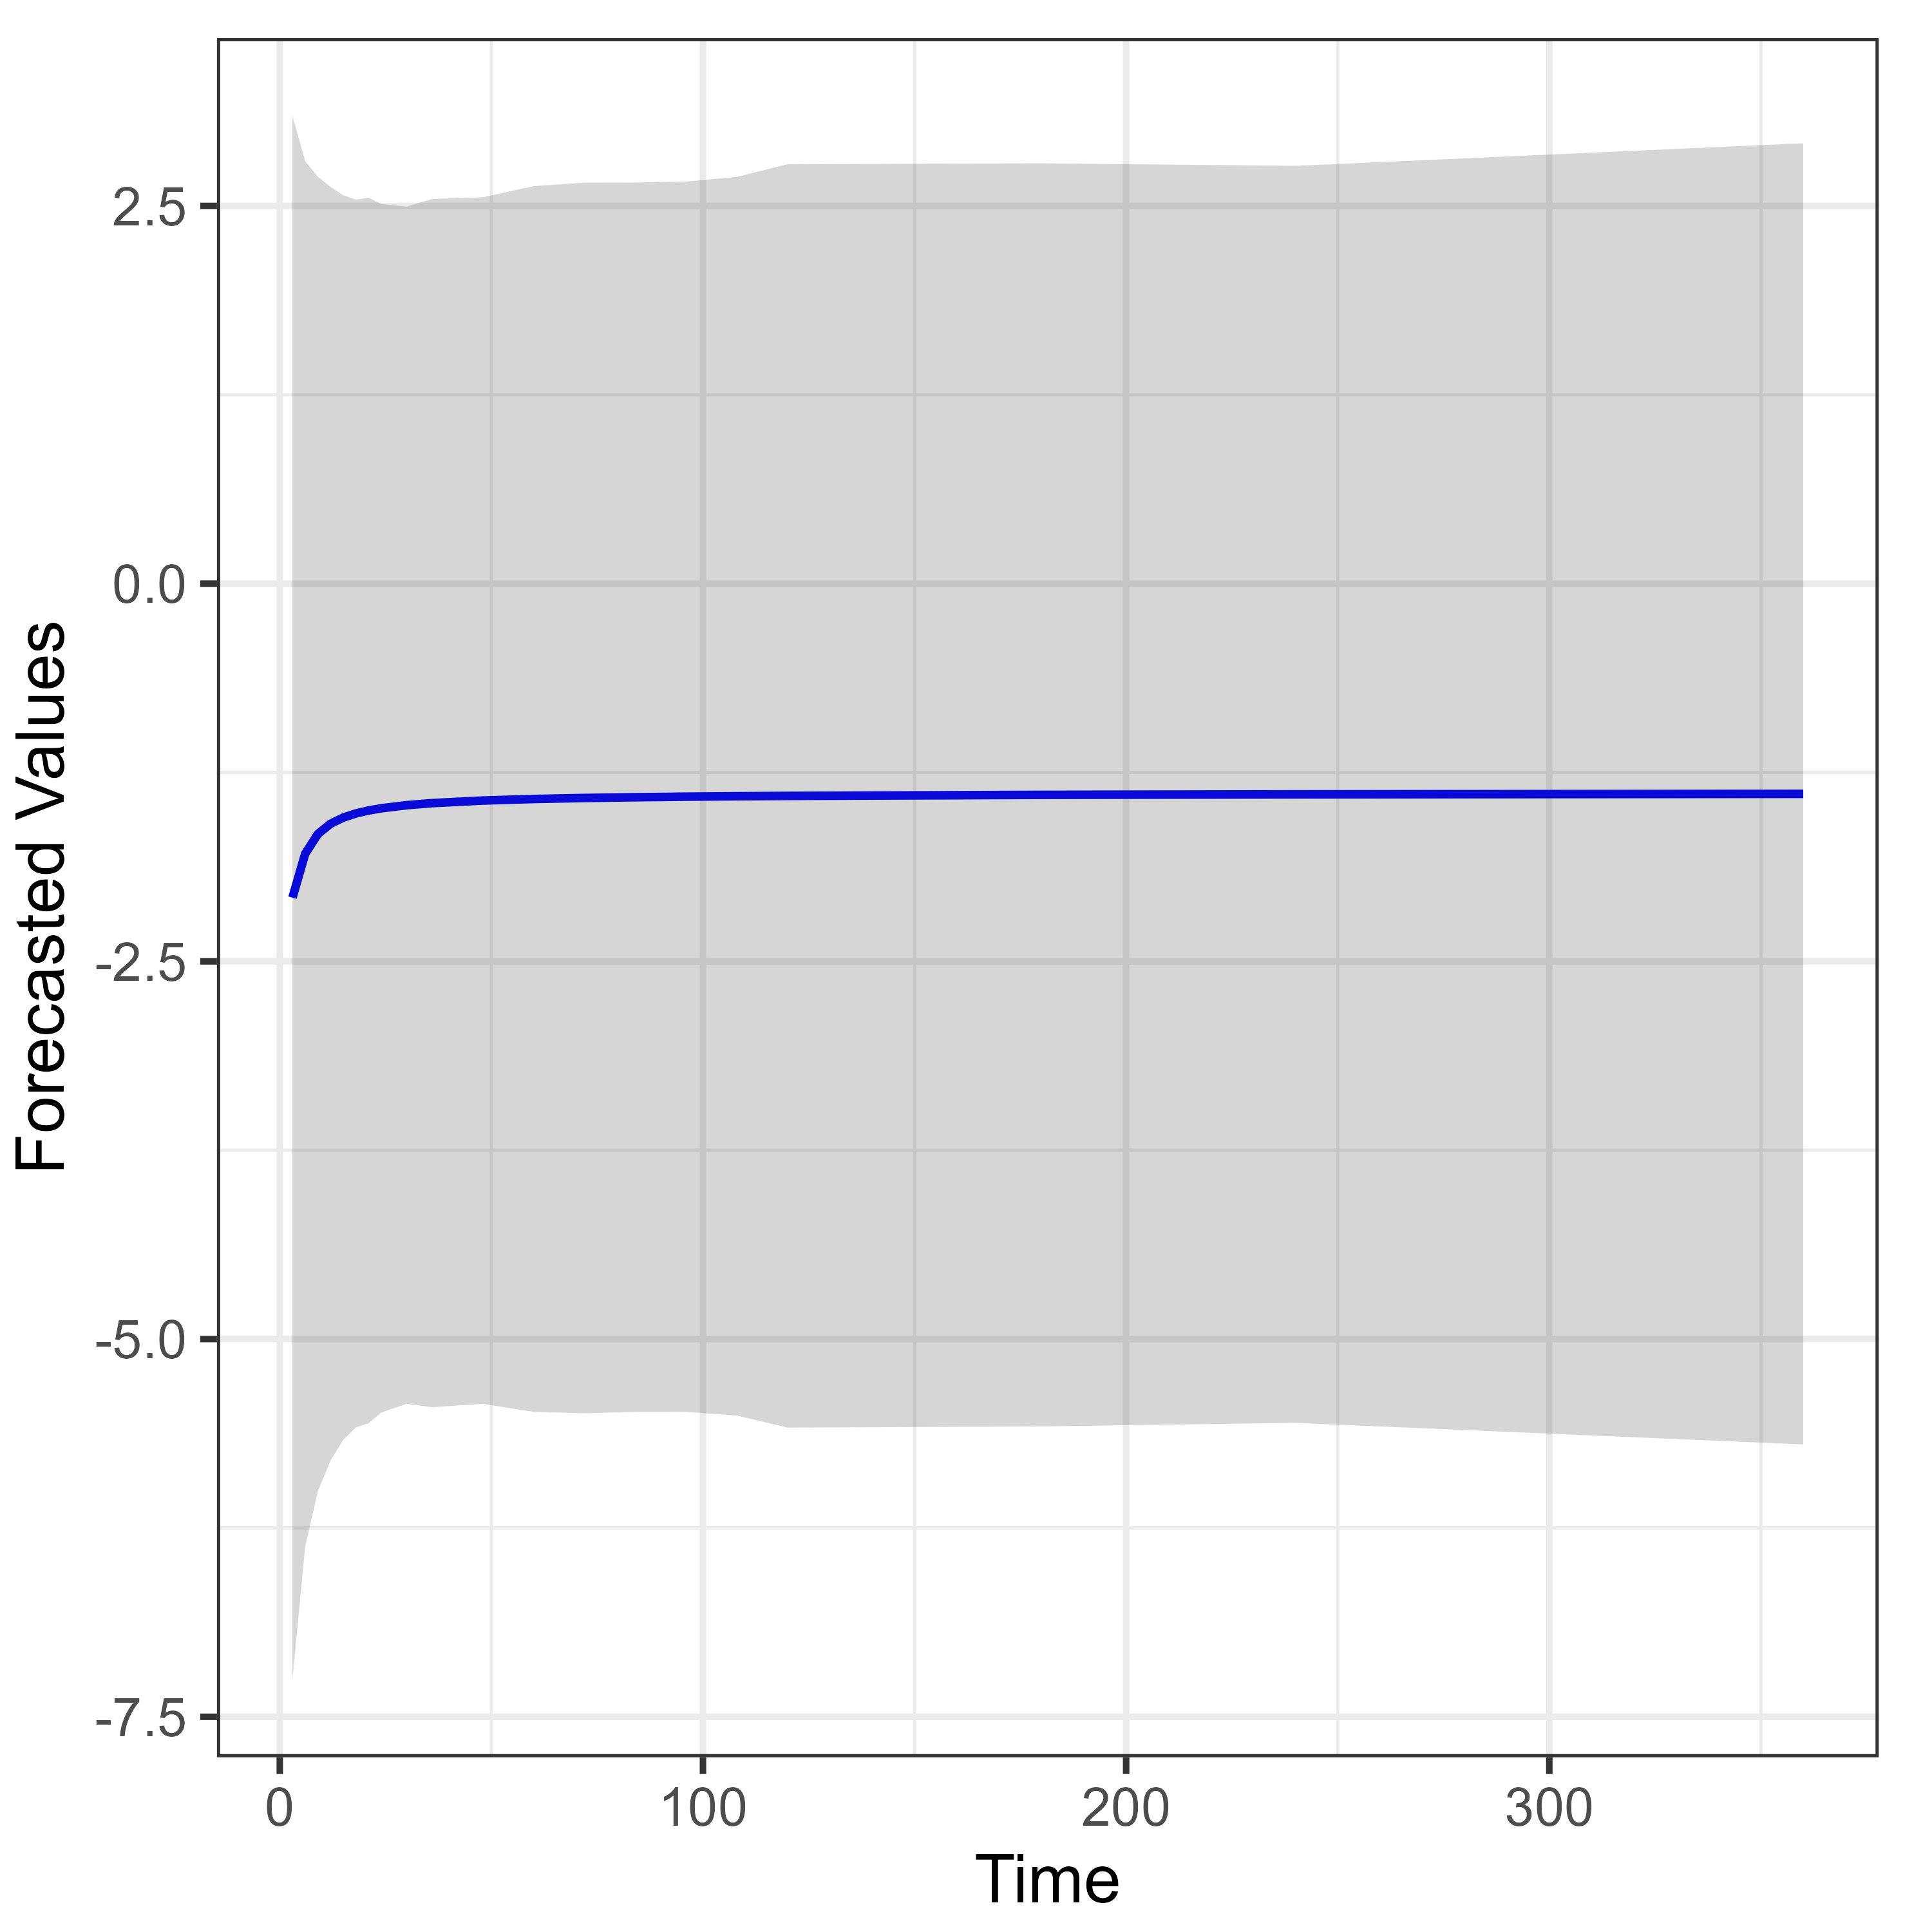
\includegraphics[width=0.9\textwidth]{../figures/forecast.png}
    \caption{Predictive yield curve with 95\% prediction intervals for maturities from 3 to 360 months.}
\end{figure}

As the uncertainty is quite large, the predictive intervals are wide, especially for longer maturities. We also plot the yield curve without the prediction intervals for understanding its shape and level.

\begin{figure}[H]
    \centering
    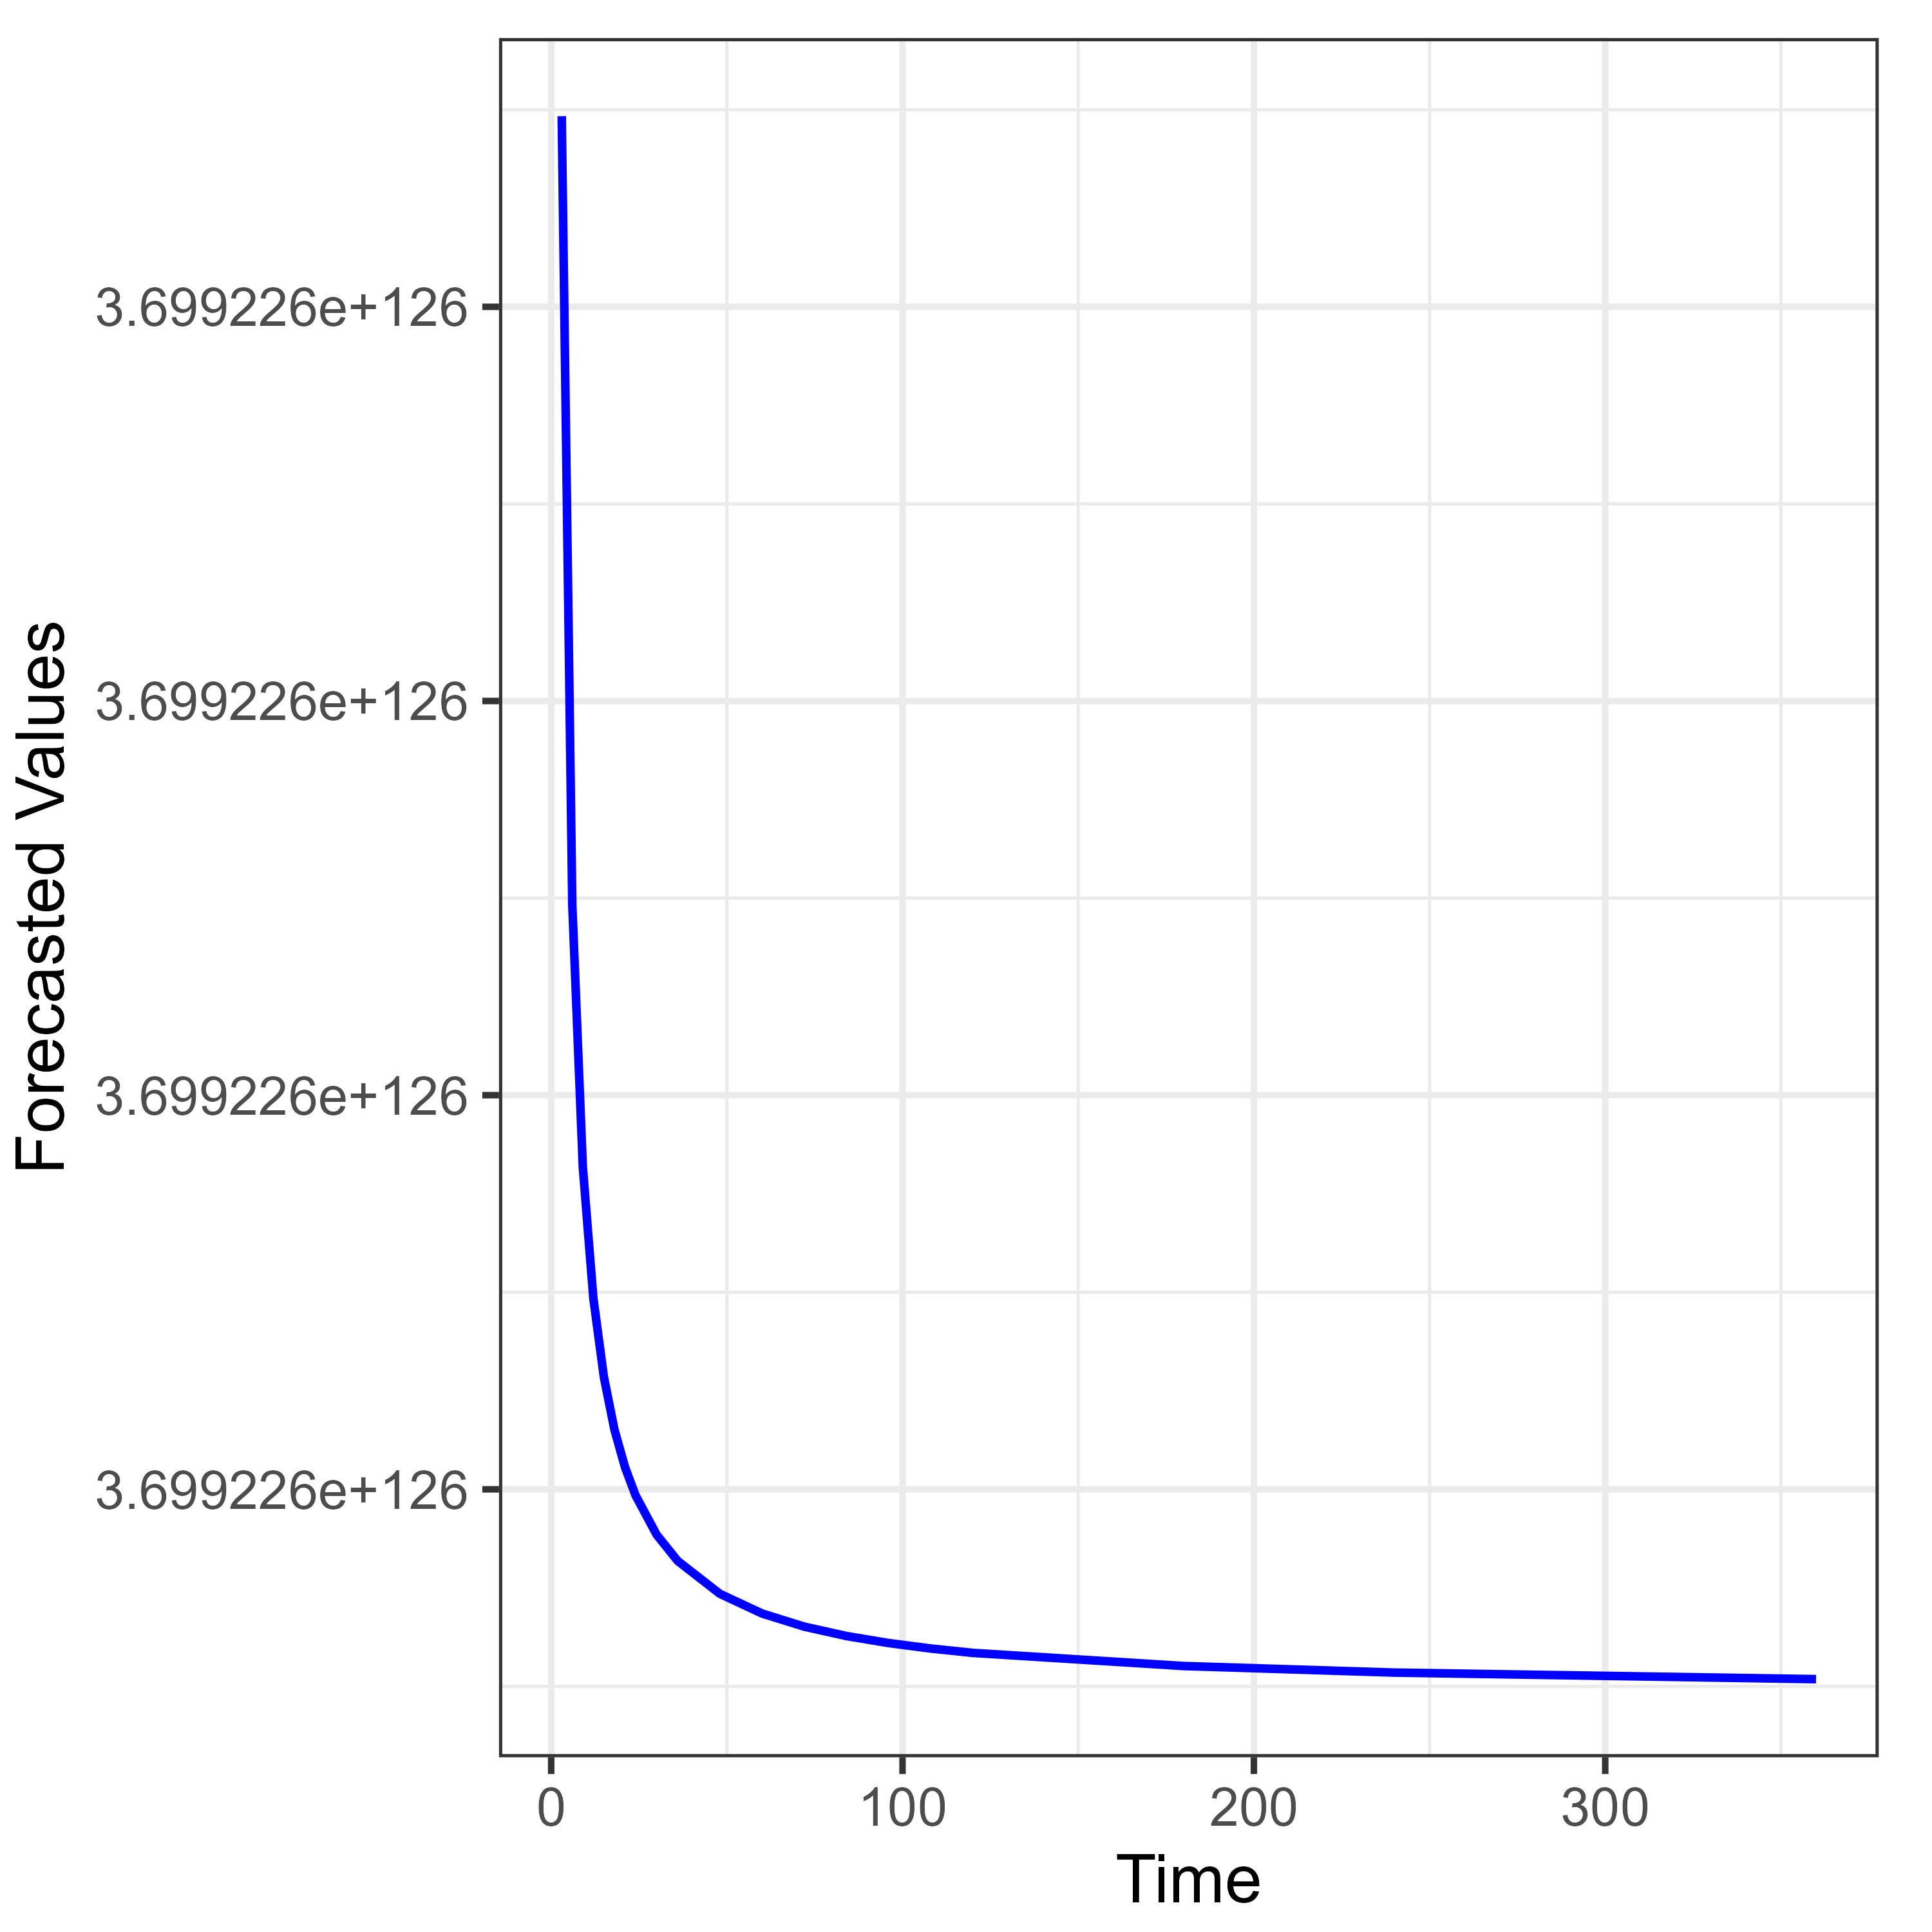
\includegraphics[width=0.9\textwidth]{../figures/forecast_no_intervals.png}
    \caption{Predictive yield curve without prediction intervals for maturities from 3 to 360 months.}
\end{figure}